\chapter{Future Work}

\section{Current State}
Our project is a working proof of concept for a successful affordable option for hearing impaired individuals. It is not  a perfect system and components have more than is needed driving up costs; however, the benefit is that we use easily available devices that others can use to build upon the product. Since Node-RED is open source, members of the community can easily add nodes that benefit from our system.

\section{Next Steps}
Since the architecture is in place, a company could build a viable product. The main missing part to our system is a completely functioning smartphone application like in Figure \ref{fig:mobile}. The purpose of the smartphone application is to abstract user control of the system. The functionality is all possible but scripts have to be made to modify the necessary parts of the Node-RED application.

\begin{figure}[h]
  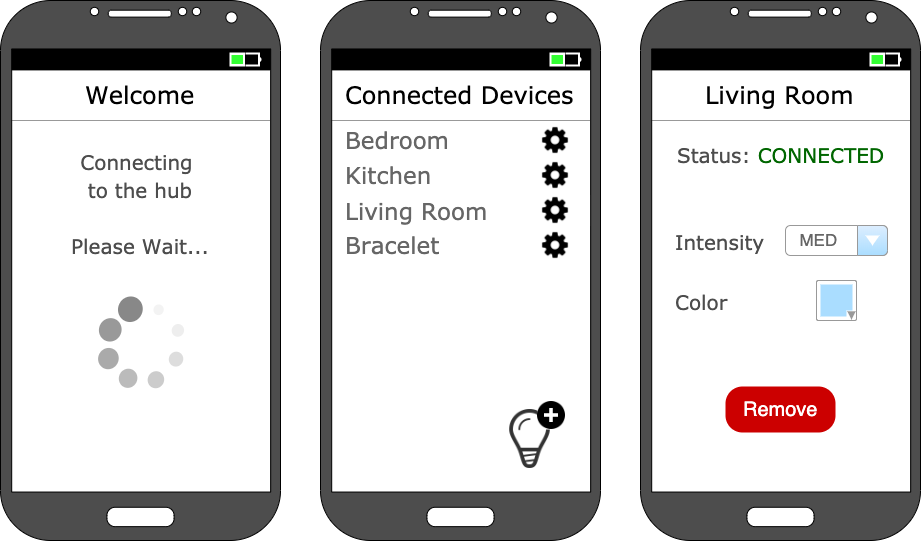
\includegraphics[width=0.8\textwidth]{Phone_App.png}
  \centering
  \caption{Mobile App Design}
  \label{fig:mobile}
\end{figure}

Another benefit would be to make a Raspberry Pi image that works directly as is. This would make it easier for users to download software for the Raspberry Pi. Our current implementation in Node-RED is already set to work on start up. More abstraction would allow this system to not only be useful for those that are familiar with the Raspberry Pi ecosystem but for the average user.